\subsection{Denominator}

\subsubsection{Lookup-table}
A big advantage of using a lookup-table is also the possibility make the data
point interval configurable. Figure \ref{fig:x-algo:non-norm} shows a
variation of implementation in figure \ref{fig:x-algo:lookup} with the
possibility of providing a custom interval.

\begin{figure}[H]
	\centering
	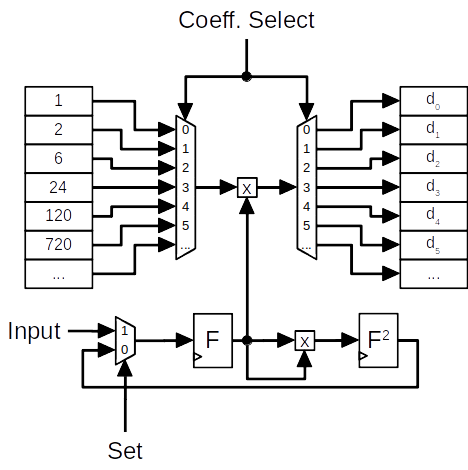
\includegraphics[width=.8\textwidth]{content/results/x-algo_lookup.png}
	\caption{Hardware algorithm to calculate the denominator with lookup-table for non-normalized intervals.}
	\label{fig:x-algo:lookup}
\end{figure}

The lookup table is a lot faster, but also uses the same amount of storage as
the dataset.

The lookup table for nine denominators is as follows:
\begin{table}[H]
	\centering
	\begin{tabular}{ c | c }
		\textbf{Index} & \textbf{Value} \\ \hline
		{\color{gray}0} & {\color{gray}1} \\
		1 & 1 \\
		2 & 2 \\
		4 & 6 \\
		5 & 24 \\
		5 & 120 \\
		6 & 720 \\
		7 & 5040 \\
		8 & 40320 \\
	\end{tabular}
	\caption{Denominator for up to column 8. Column \textit{0} contains the \textit{y} values.}
\end{table}


\subsubsection{On-the-fly generation}
As mentioned a lookup table requires a lot of storage. One way of mitigating
this problem is at the cost of speed and die space. Figure
\ref{fig:x-algo:on-the-fly} shows the hardware implementation for a on-the-fly
generation of the denominators.

\begin{figure}[H]
	\centering
	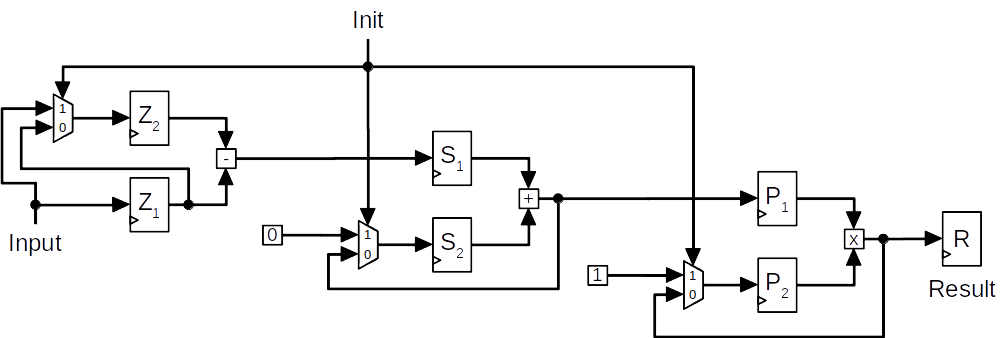
\includegraphics[width=.8\textwidth]{content/results/x-algo_on-the-fly.png}
	\caption{Hardware algorithm to calculate the denominator consecutively.}
	\label{fig:x-algo:on-the-fly}
\end{figure}
